%%%%%%%%%%%%%%%%%%%%%%%%%%%%%%%%%%%%%%%%%%%%%%%%%%%%%%%%%%%%%%%%%%%%%%%%%%%%%%%%
%theory.tex: Chapter on light dark matter theory
%%%%%%%%%%%%%%%%%%%%%%%%%%%%%%%%%%%%%%%%%%%%%%%%%%%%%%%%%%%%%%%%%%%%%%%%%%%%%%%%
\chapter{Theory}
\label{theory}
%%%%%%%%%%%%%%%%%%%%%%%%%%%%%%%%%%%%%%%%%%%%%%%%%%%%%%%%%%%%%%%%%%%%%%%%%%%%%%%%
\section{Thermal Dark Matter}
The core principle of thermal dark matter models, like the one presented here, is that for some period of time in the early universe dark matter is in thermal equilibrium with standard model matter.
This thermal equilibrium is achieved to due the high temperature and density of the early universe, where despite small SM couplings dark matter particles can be frequently produced through interactions with standard model particles and produce standard model particles through their own interactions and decays.
As the early universe expands and cools, the rate of these interactions decreases until the dark matter interaction rate fall below the Hubble expansion rate and "freezes out", leaving thermal equilibrium with SM matter and leaving its phase-space distribution subject only to the universe expansion and eventual structure formation \cite{ref:thermalDM}.


\section{Light Dark Matter}

\section{Targeting Dark Matter Production}
If a light dark matter coupling were present, there are several potential signatures that could appear in an experiment like CMS.

Traditional searches in CMS look for particle production in the initial scattering process between proton constituents.
As a light dark matter coupling would allow mixing between the \aprime and any standard model photon, dark matter could be produced in initial state collisions with electromagnetic interactions between partons that produce photons that then mix with the \aprime.

Unfortunately, decays of the \aprime outside of the detector or into other dark matter particles which are invisible to CMS make this initial production mode very difficult to distinguish.
Events with large initial state radiation from the partons can make this signal visible as a large missing transverse momentum in the event, but the large reduction in acceptance from this type of requirement causes the resulting limit to be very weak.

Instead of searching for dark matter production in the initial state, the signal could appear in a secondary interaction between a final state particle and the detector itself.
The relatively small masses of light dark matter particles limits the loss in the interaction rate due to the much lower center of mass energy in these secondary interactions compared to the initial collision, and the high particle flux and large size of the detector result in a significant fixed target luminosity.

The primary signature of a secondary interactions between a particle emitted from the initial collision and the detector would be missing energy carried by the invisible \aprime and a change in the trajectory of the visible particle.
These types of signatures are difficult to observe in particles with have large standard model interaction rates, as the shower of particles produced in their interactions can lead to large uncertainties in their energy measurement and little hope of observing trajectory differences.
In addition, high interaction rates expose particles to less of the detector as they are stopped relatively quickly, reducing the effective luminosity.

For these reasons, the selections in this search target potential dark matter interactions of final state muons.
As muons have small standard model cross sections they lose very little energy while they traverse the detector, leading to high consistency in projecting their trajectory and observing potential changes, as well as low rates of stopped muons due to standard model processes which could fake the energy loss to an \aprime.

With a light dark matter mixing, muons would primarily produce dark matter in the mass ranges of interest via a process known as \dbrem, where a dark matter particle is emitted from a muon as it recoils from the electromagnetic field of a nucleus in the detector (\Cref{fig:dbrem_feyn}).
While other processes, such as photoproduction of vector mesons which then decay invisibly through dark matter coupling, would also be present with the assumed coupling, only \dbrem is considered in this search due to its significantly larger production rate.

\include{figure}[ht]
	\centering
	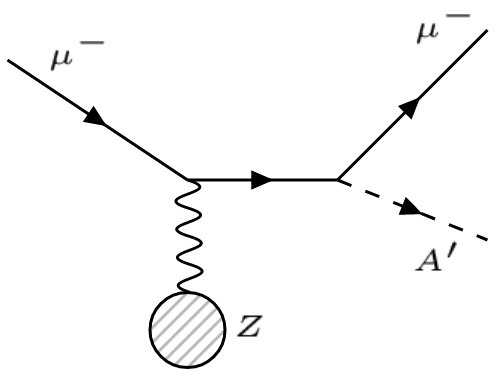
\includegraphics[width=\textwidth]{figures/dbrem_feyn_diagram.jpg}
        \caption[Dark Bremmstrahlung Feynman Diagram]{Dark Bremsstrahlung caused by a muon interacting with a nucleus with atomic number Z.}
\end{figure}

As an additional feature of muon-initiated \dbrem, results from this search are also sensitive to dark matter models which replace the generic dark matter mixing with an asymmetric coupling to the lepton generations.
While lepton universality is built into the standard model, no such requirement is necessary for new physics models. 

There are several experimental anomalies which could potentially be explained by an asymmetric lepton coupling of this type.
The measurement of the muon magnetic moment by the Fermilab E989 experiment \cite{gminus2}, combined with the original result from Brookhaven \cite{gminus2_bnl} leads to a 4.2 $\sigma$ discrepancy with the theoretical prediction \cite{gminus2_theory}. 
This could potentially be explained by a dark matter signal which preferentially couples to muons, as the dark matter coupling would alter the muon magnetic moment through additional loop diagrams.

\section{Z-Bosons and the DY Process}
%%%%%%%%%%%%%%%%%%%%%%%%%%%%%%%%%%%%%%%%%%%%%%%%%%%%%%%%%%%%%%%%%%%%%%%%%%%%%%%%
